\documentclass{article}

% Language setting
% Replace `english' with e.g. `spanish' to change the document language
\usepackage[english]{babel}

% Set page size and margins
% Replace `letterpaper' with `a4paper' for UK/EU standard size
\usepackage[letterpaper,top=2cm,bottom=2cm,left=3cm,right=3cm,marginparwidth=1.75cm]{geometry}

% Useful packages
\usepackage{amsmath}
\usepackage{graphicx}
\usepackage[colorlinks=true, allcolors=blue]{hyperref}

\title{COS 720 Project}
\author{Tiyego Emito Khoza (u20665777)}

\begin{document}
\maketitle

\section{Research}

\subsection{Cloud Security}
THe cloud is a vast ecosystem. Basically someone else's computer, and it comes in many shapes and sizes so we have to be able to set up protections for it

\subsection{History}
The website link was \href{www.wikispaces.com}{www.wikispaces.com}. The platform was developed by Tangient LLC in March 2005. It became one of the most popular wiki hosts, in particular it was used for educational purposes primarily with Grade K - 12. This led to it being acquired by Tes Global in 2014.

The platform lost popularity after dropping its free servers only allowing educational content for non premium users in 2014. It's usage and maintaince became difficult which led to a blog post \cite{GoodbyeWikispaces}

\subsection{Target Industry}
Wikispace was made for general purpose but it mostly caught traction in the education sector \cite{WhereToNext}

\subsection{Strengths, Weaknesses and Improvements}
Wikispaces has somethings I'd like to talk about

\subsubsection{Strengths}
One of the beloved features of Wikispaces  was the face that it was easy to use, making it popular choice for education apps. It's simple to use interface was easy to follow \cite{WikispacesTutorial}. It was structured and organized, access control was effective and it being free was what put it ahead of the market

\subsubsection{Weaknesses}
Wikispaces was far too simple, so much so that it was hard to add improvements on its interface and it wasn't very good on mobile. It did not help for them to start making the application

\subsubsection{Improvements}
The improvements could be made on its design, and improved performance. Also expanding all of its features and some new features were proposed even after it died. \cite{CreateWikiWithWordPress}

\section{Software Requirements Specification}

\subsection{Introduction}

The purpose of Wikispaces was to provide a simple interface for the creation and management for people with others wanting to make wikis or website pages for their projects or note keeping. \newline

Most of the design decisions focused around being user friendliness and productivity with its collaboration tools. It's focus on basic design and appearance limited most of its functionality, so the learning curve wasn't too high and managing the content was relatively simple. \newline

Because of this, Wikispaces became one of the popular applications. But its business requirements were not being met, as the competition was a bit too overbearing and the shift to the mobile was something they were not ready for.

\subsection{User Characteristics}

The main demographic for Wikispaces was a broad audience, it's focus shifted to being a good education tool \cite{WikispacesClosedDown}. Here are the types of users and their skills

Users should be interested in creating and managing wikis. Another set of users who would like to create and edit pages for wikis. And there's the casual user who would like to view the content and find what they need.

\subsubsection{Admins}
These are users with administrative control each their entire wiki. A person is an admin if they are either assigned that role or created the Wiki space

\begin{itemize}
    \item Admins are the users who want to create and manage Wiki
    \item Admins add, remove or ban users from the application
    \item Admins can customize the wiki page from the theme to the title
    \item Admins set policies for page creation
    \item Admins can assign user roles and permissions
\end{itemize}

\subsubsection{Editors}
Editors are the content creators for pages, they can either be one or many

\begin{itemize}
    \item Editors would like to write content on pages
    \item Editors would like to upload media files 
\end{itemize}

\subsubsection{Viewers}
A viewer is someone who'd like to view the content, they normally wouldn't need an account if viewing public Wiki and pages.

\begin{itemize}
    \item Viewers only need read only access to the pages they allowed
    \item May or may not need to be authenticated
\end{itemize}

\subsection{Functional requirements}
Specify functional requirements to satisfy the use cases. Formulate them in terms of requirements

The use cases will be based on the user characteristics and features listed before. The function

\begin{itemize}
    \item[\textbf{R.1}] Wiki Creation and Access Management
    \begin{itemize}
        \item[\textbf{R.1.1}] Users shall be able to create wikis for groups.
        \item[\textbf{R.1.2}] Users shall be able to define access levels for each wiki.
    \end{itemize}
    
    \item[\textbf{R.2}] User Permissions
    \begin{itemize}
        \item[\textbf{R.2.1}] Users shall be able to set permissions for creating pages.
        \item[\textbf{R.2.2}] Users shall be able to set permissions for editing pages.
        \item[\textbf{R.2.3}] Users shall be able to set permissions for viewing pages.
    \end{itemize}
    
    \item[\textbf{R.3}] Page Editing
    \begin{itemize}
        \item[\textbf{R.3.1}] Users shall be able to edit existing pages.
        \item[\textbf{R.3.2}] Users shall be able to create new pages.
        \item[\textbf{R.3.3}] Users shall be able to edit the content on pages.
    \end{itemize}
    
    \item[\textbf{R.4}] Revisions and Navigation
    \begin{itemize}
        \item[\textbf{R.4.1}] Users shall be able to view and revise changes in pages.
        \item[\textbf{R.4.2}] Users shall be able to navigate between pages within a wiki.
    \end{itemize}
    
    \item[\textbf{R.5}] Discussions and Notifications
    \begin{itemize}
        \item[\textbf{R.5.1}] Users shall be able to create discussion pages associated with each page.
        \item[\textbf{R.5.2}] Users shall be able to send comments on discussion pages.
        \item[\textbf{R.5.3}] Users shall be able to set notifications for pages after they've been modified.
    \end{itemize}
    
    \item[\textbf{R.6}] Media and Organization
    \begin{itemize}
        \item[\textbf{R.6.1}] Users shall be able to upload images and multimedia to the pages they create.
        \item[\textbf{R.6.2}] Users shall be able to assign categories to pages.
    \end{itemize}
    
    \item[\textbf{R.7}] Exporting
    \begin{itemize}
        \item[\textbf{R.7.1}] Users shall be able to export their wiki pages and content into multiple file formats (HTML, PDF, DOCX, etc.).
    \end{itemize}
    
    \item[\textbf{R.8}] Customization
    \begin{itemize}
        \item[\textbf{R.8.1}] Users shall be able to customize the appearance of their wikis.
    \end{itemize}
\end{itemize}

\subsection{Use Case Diagram}

\subsubsection{User Wiki Management}
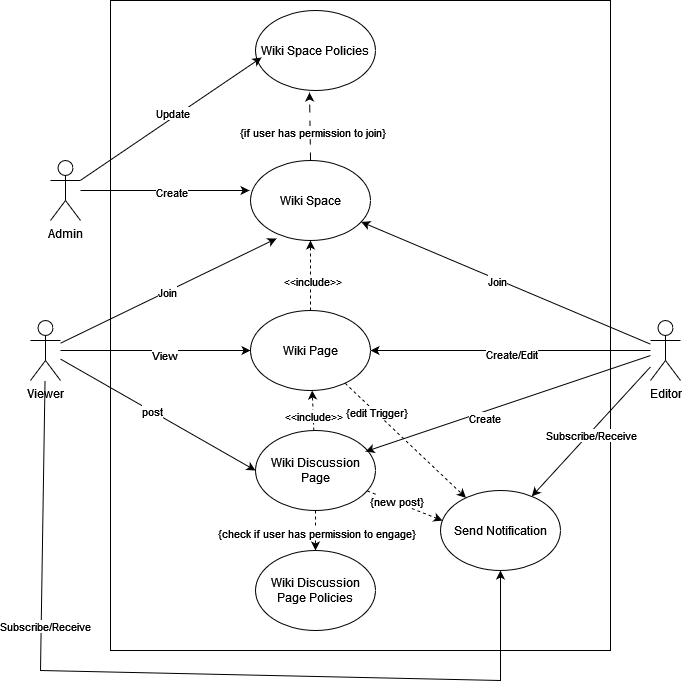
\includegraphics[width=\textwidth]{User-Wiki-Management.png}

\subsection{Traceability Matrix - Requirements VS Sub-systems}

A matrix

\subsection{Component/Class diagram model}

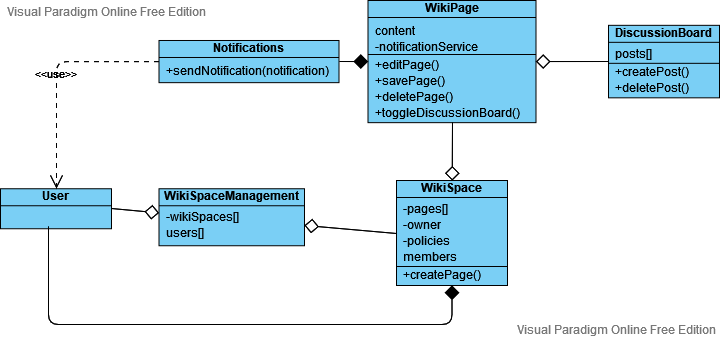
\includegraphics[width=\textwidth]{Class Diagram.png}

\subsection{Non-Functional Requirements (Quality requirements)}

Wikispaces is rich full of features, and we want the following qualities for each:\dots

\subsubsection{Usability}

The system should be simple and well designed, not overly complicated. The users should not feel overwhelmed and find it to be a easy process to find their designed Wikis and view the content. And also editing the content. To accomplish this, careful consideration should be made towards making a nice UI and should be tested with a Usability test so that the UI can be improved with real user feedback.

\subsubsection{Availability}

The system should always be available for users, they need to be able to access their content in a timely manner, the desired being 99\% of the time. To achieve this, the website would have to make use of reliable cloud platform which provides servers for hosting with backup plans

\subsubsection{Scalability}

The system should be able to handle both a large number of users and their operations. They'll be continuously fetching data from the server to view, edit, moderate and multiple other operations, so it should be possible to handle 900-1000 requests at a time. The servers used should be high quality, which would be expensive so the right architecture would have to be picked.

\subsubsection{Security}

The security of the content hosted is of the up most importance the system's access control and user roles should be well defined and built properly according to security standards. Admins would trust their private wiki shouldn't be accessible by anyone they haven't authorized.

\subsection{Conclusion}
That concludes our document thank you

\bibliographystyle{alpha}
\bibliography{sample}

\end{document}